\section{Resultados}

	Como afirmado anteriormente, o primeiro passo do projeto é a prototipagem do Hardware do sistema, que inclui o Arduino, os botões e potenciômetros, através da plataforma online TinkerCAD, que inclui em si um monitor serial para visualizar o que está sendo enviado serialmente pelo microcontrolador.

\begin{figure}[htbp]
     \centerline{
        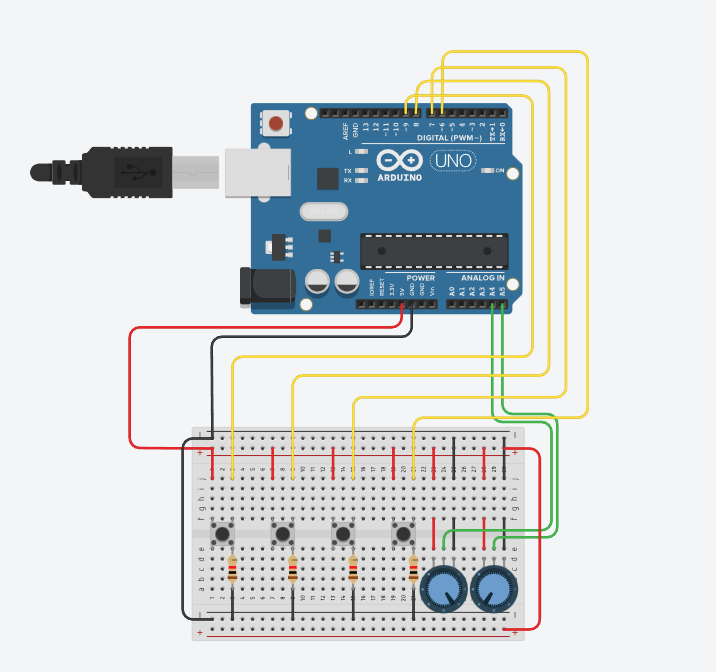
\includegraphics[width=3in]{tinkercad.png}
        }
     \caption{Modelo prototipado no TinkerCAD.}
     \label{fig}
    \end{figure}

	Como pode ser visto na figura acima, o modelo foi criado para abrigar dois potenciômetros e uma quantidade de botões, que foram 4 no momento da simulação. Cada um destes associados a um pino digital respectivo. Assim, a função do Arduino será pegar as informações desses componentes eletrônicos e enviar serialmente para o computador serialmente. O que tornará isso possível é a utilização da biblioteca "softwareserial.h" e suas funções, que possibilitam a comunicação.
	
	Para enviar todas as informações de uma única vez, em um pacote só, elas serão inseridas em uma string, e sua separação será realizada no código do Processing. Assim sendo, o código inserido no Arduino compreende a seguinte lógica:

\begin{lstlisting}[language=C]
const int pot1 = A5, pot2 = A3; //Potenciometros
const int b01 = 8, b02 = 7; // Botoes
int v_pot1 = 0, v_pot2 = 0; //Valores dos potenciometros
bool v_b01,v_b02; //Valores dos Botoes
int arr[10];

void setup() {
  Serial.begin(9600);
  pinMode(pot1, INPUT);
  pinMode(pot2, INPUT);
  
  for(int i = 7; i <= 8; i++){
      pinMode(i, INPUT_PULLUP);
    }
}

void loop() {
  v_pot1 = map(analogRead(pot1),0,1023,0,255);
  Serial.print(String(v_pot1) + "-");
  
  v_pot2 = map(analogRead(pot2),0,1023,0,255);
  Serial.print(String(v_pot2) + "-");
  
  v_b01 = !digitalRead(b01);
  v_b02 = !digitalRead(b02);

  Serial.print(String(v_b01) + "-");
  Serial.print(String(v_b02) + "\n");
  delay(50);
}
\end{lstlisting}

	Além da declaração de variáveis, alguns recursos foram utilizados para saber por exemplo, se um botão estava sendo pressionado. Como ele está pinado em uma porta digital, é possivel utilizar uma propriedade chamada "INPUT\_PULLUP"	para fazer essa distinção. Isso ocorre já que o botão está conectado a um resistor de "Pull-Up", que está inbutido no Arduino UNO, e quando vemos a expressão abaixo, significa que essa resistência irá impactar naquele input quando acionado, atuando como um inversor, para assim se obter um nível lógico alto quando o botão é pressionado:

\begin{lstlisting}[language=C]
pinMode(i, INPUT_PULLUP);
\end{lstlisting}

	Outra lógica notável é que as informações a serem enviadas, dois associados aos potenciômetros e outros dos botões, serão colocadas em uma string única. Na função "loop" do Arduino, observa-se que é exatamente isso que está ocorrendo, criando uma string de modelo "[x-x-x-x]", que é um pacote de informações que será enviado ao processing, e lá será transformado em um vetor de caracteres, e a associação é feita utilizando um artefato chamado "this". Esse operador atribui um valor a uma classe, e essa única classe apenas, evitando que esta fosse para outra classe indesejada.

\begin{lstlisting}[language=Java]
class bot {
  String frase = "";
  int px, py;
  float tamanho = 0;
  int r = 0, g = 0, b = 0;
  
  void setColor(int r, int g, int b) {
     this.r = r;
     this.b = b;
     this.g = g;
  }

  bot(int px, int py) {
    this.px = px;
    this.py = py;
  }

  void escreve(String frase) {
    textSize(height/12.5);
    tamanho = textWidth(frase);
    
    //fill(r,g,b);
    fill(220, 80, 80);
    rect(this.px, this.py+15, tamanho+50, 120, 28);
    textAlign(CENTER, CENTER);

    fill(0);
    text (frase, this.px, this.py);
  }

  void select_bot() {
    stroke(225);
    fill(225, 225);
    rect(px, py+15, tamanho+80, 80, 28);
  }
}
\end{lstlisting}

	%%explicação do uso do this aqui

	%%explicação do código aqui

	%% falar dos controles impressos 3D

	%% foto do Jogo


%% dois fios para conectar um botão
%% comunicação transformar um string em um array de caracteres e leu os valores individualmente
%% precisava uma coisa chamada "this" como seletor restingir informações à uma classe
